\section{\gsnfs{} Overview}\label{sec:design-overview}

\begin{outline}
  \textbf{Page budget: 1 page} \status{[Done]}

  Background: \status{[Done]}
  \begin{itemize}
  \item 3D Gaussians: introduce positions, and other attributes; make sure we briefly explain the various attributes
  \item Briefly describe what it means to apply compression techniques: i.e., to generate a bitstream from these (maybe use a figure)
  \end{itemize}

  Key idea: \status{[Done]}
  \begin{itemize}
  \item Entirely GPU-based implementation
  \end{itemize}

  Requirements: all components should be GPU-resident to avoid memory copy costs
  
  Include figure of different components and how they related: describe what each component does (like the design figure in LiVO). \status{[Done]}
  \begin{itemize}
  \item Include rendering in the figure, but omit description afterwards
  \end{itemize}
  
\end{outline}

\gsnfs is designed as a fast, post-training volumetric video codec that enables on-demand streaming of photo-realistic 3D scene. Every frame of a volumetric video is represented as a 3D Gaussian Splatting (3DGS) model, which consists of a large number of 3D Gaussians, each defined by its 3D position and a set of rendering attributes. Though 3DGS has been shown to achieve superior visual quality compared to other volumetric representations, it also results in a massive data footprint, making it challenging to stream over mobile networks.

Each 3DGS model is represented as a collection of $N$ 3D Gaussians. Unlike point clouds that store discrete $(x,y,z)$ coordinates, each Gaussian is an ellipsoid defined as following:
\begin{itemize}
\item Mean ($\mu \in \mathbb{R}^3$): This represents the position of the Gaussian in 3D space as center of the ellipsoid.
\item Scales ($s \in \mathbb{R}^3$): This defines the size of the ellipsoid along its three axes.
\item Rotation ($q \in \mathbb{R}^4$): This defines the orientation of the ellipsoid in 3D space, typically represented as a quaternion.
\item Opacity ($\alpha \in \mathbb{R}$): This represents the transparency of the Gaussian.
\item Colors ($c$): Colors are represented as spherical harmonics (SH) of varying degrees. The SH coefficient of degree $d = 0$ represents the color of the Gaussian, often referred to as DC. The higher degree SH coefficients of degree $d > 0$ capture more complex view-dependent lighting and shading effects, often referred to as AC coefficients. The number of color attributes is given by $3 + 3 * (d + 1))^2$, where the first 3 are the DC and rest are AC coefficients, respectively. For example, a common choice of SH degree is 3, which results in $48$ color attributes per Gaussian.
\end{itemize}

A typical full scene in a volumetric video can consist of \note{XXX} Gaussians. If each Gaussian is represented with SH degree 2, then the total number of attributes per Gaussian is $3 + 3 + 4 + 1 + 48 = 59$. With each attribute represented as a 32-bit floating point number, this results in uncompressed size of \note{XXX}~MB per frame. This is prohibitively large for streaming over broadband and  mobile networks with typical bandwidths in the range of \note{XX-XXX} Mbps. Therefore, effective compression techniques are essential to reduce the data size while maintaining visual quality.

Unlike a point cloud or mesh which has geometry and color/texture, compressing a 3DGS frame is non-trivial since it has a more complex structure with multiple attributes. Each attribute needs to be carefully encoded. For example, any loss in the geometry of a 3DGS represented by position, scales, and rotations, will result in distorted visual artifacts. Similarly, the color information is not just RGB values, but also includes higher order SH coefficients and opacity. Any compression technique needs to encode all these attributes in a compact binary bitstream, which can be transmitted from server to client, and then decoded back to a 3DGS model for rendering.

3DGS is trained in the server on Graphical Processing Units (GPUs) using CUDA, which allows for efficient parallel processing of the large number of Gaussians. Similarly, the client also uses GPU for rendering the 3DGS frames. Therefore, to avoid costly memory copy between CPU and GPU, it is critical that the entire encoding and decoding pipeline of \gsnfs is implemented on the GPU. This allows us to achieve low latency encoding and decoding on both server and client. Traditional 3D codecs such as Draco and G-PCC are implemented in CPU due to lack of parallelization. Using these codecs would require copying hundreds of megabytes across the PCIe bus to/from the host memory, encoding/decoding after training or before rendering.

\begin{figure}[t]
  \centering
  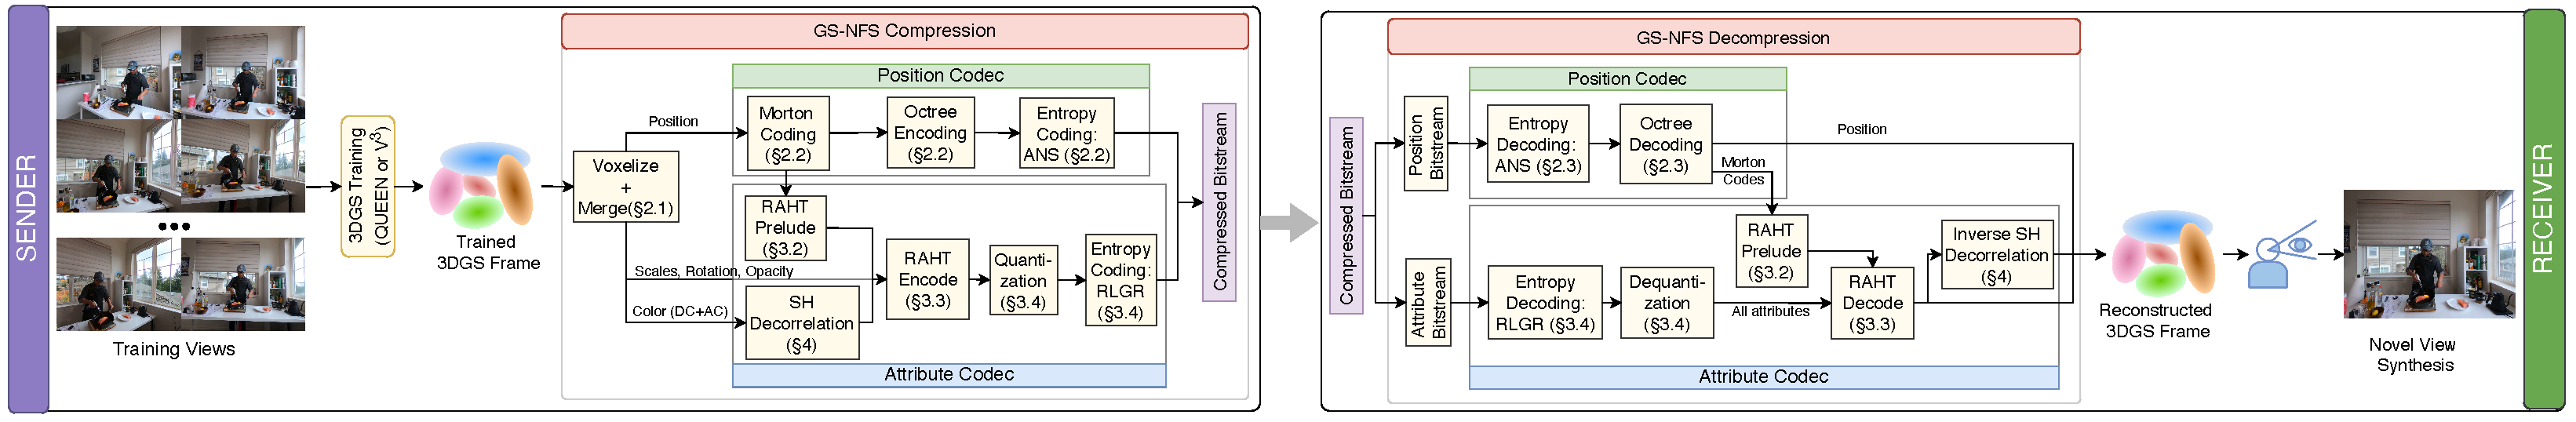
\includegraphics[width=\columnwidth]{figures/architecture.pdf}
  \caption{\gsnfs Architecture. Blocks in yellow are GPU-resident components.}
  \label{fig:architecture}
\end{figure}

